\documentclass{beamer}
\usepackage{lmodern}
\usepackage[utf8]{inputenc}

\usepackage{enumerate}
\usepackage{multimedia}
\usepackage{bbm}
\usepackage{booktabs}
\usepackage{caption}

\usetheme{polimix}

%My commands
\newcommand{\expect}[2]{\mathop{E}_{#1}\left[#2\right]}
\newcommand{\hold}{\addtocounter{framenumber}{-1}}
\newcommand{\jump}{\addtocounter{framenumber}{1}}
\newcommand{\norm}[2][\infty]{\left\|#2\right\|_{#1}}
% % % %
 
\title[Short title]{Long title}
\subtitle{subtitle}

\title[Retrace]{Retrace($\lambda$)}
\subtitle{Temporal Credit Assignment in Off-Policy Reinforcement Learning}

\author[Matteo Papini]{Matteo Papini}
\date[28/11/17]{28th November 2017}

\begin{document}

%%%%%%%%%%%%%%%%%%%%%%%%%%%%%%%%%%%%%%%%%%%%%%%%%%%%%%%%%%%%%%%%%%%%%%%%%%%%%%%%%%%%%%%%%%%%%%%%%%%%%%%%%%%%%%%%%%%%

\begin{frame}
\titlepage
\end{frame}

\addtocounter{framenumber}{-1}

%%%%%%%%%%%%%%%%%%%%%%%%%%%%%%%%%%%%%%%%%%%%%%%%%%%%%%%%%%%%%%%%%%%%%%%%%%%%%%%%%%%%%%%%%%%%%%%%%%%%%%%%%%%%%%%%%%%%

\begin{frame}
\frametitle{Before we start...}
\only<1>
{ACAI Summer School on Reinforcement Learning

Nieuwpoort, Belgium, 7-14 October 2017 
\centering
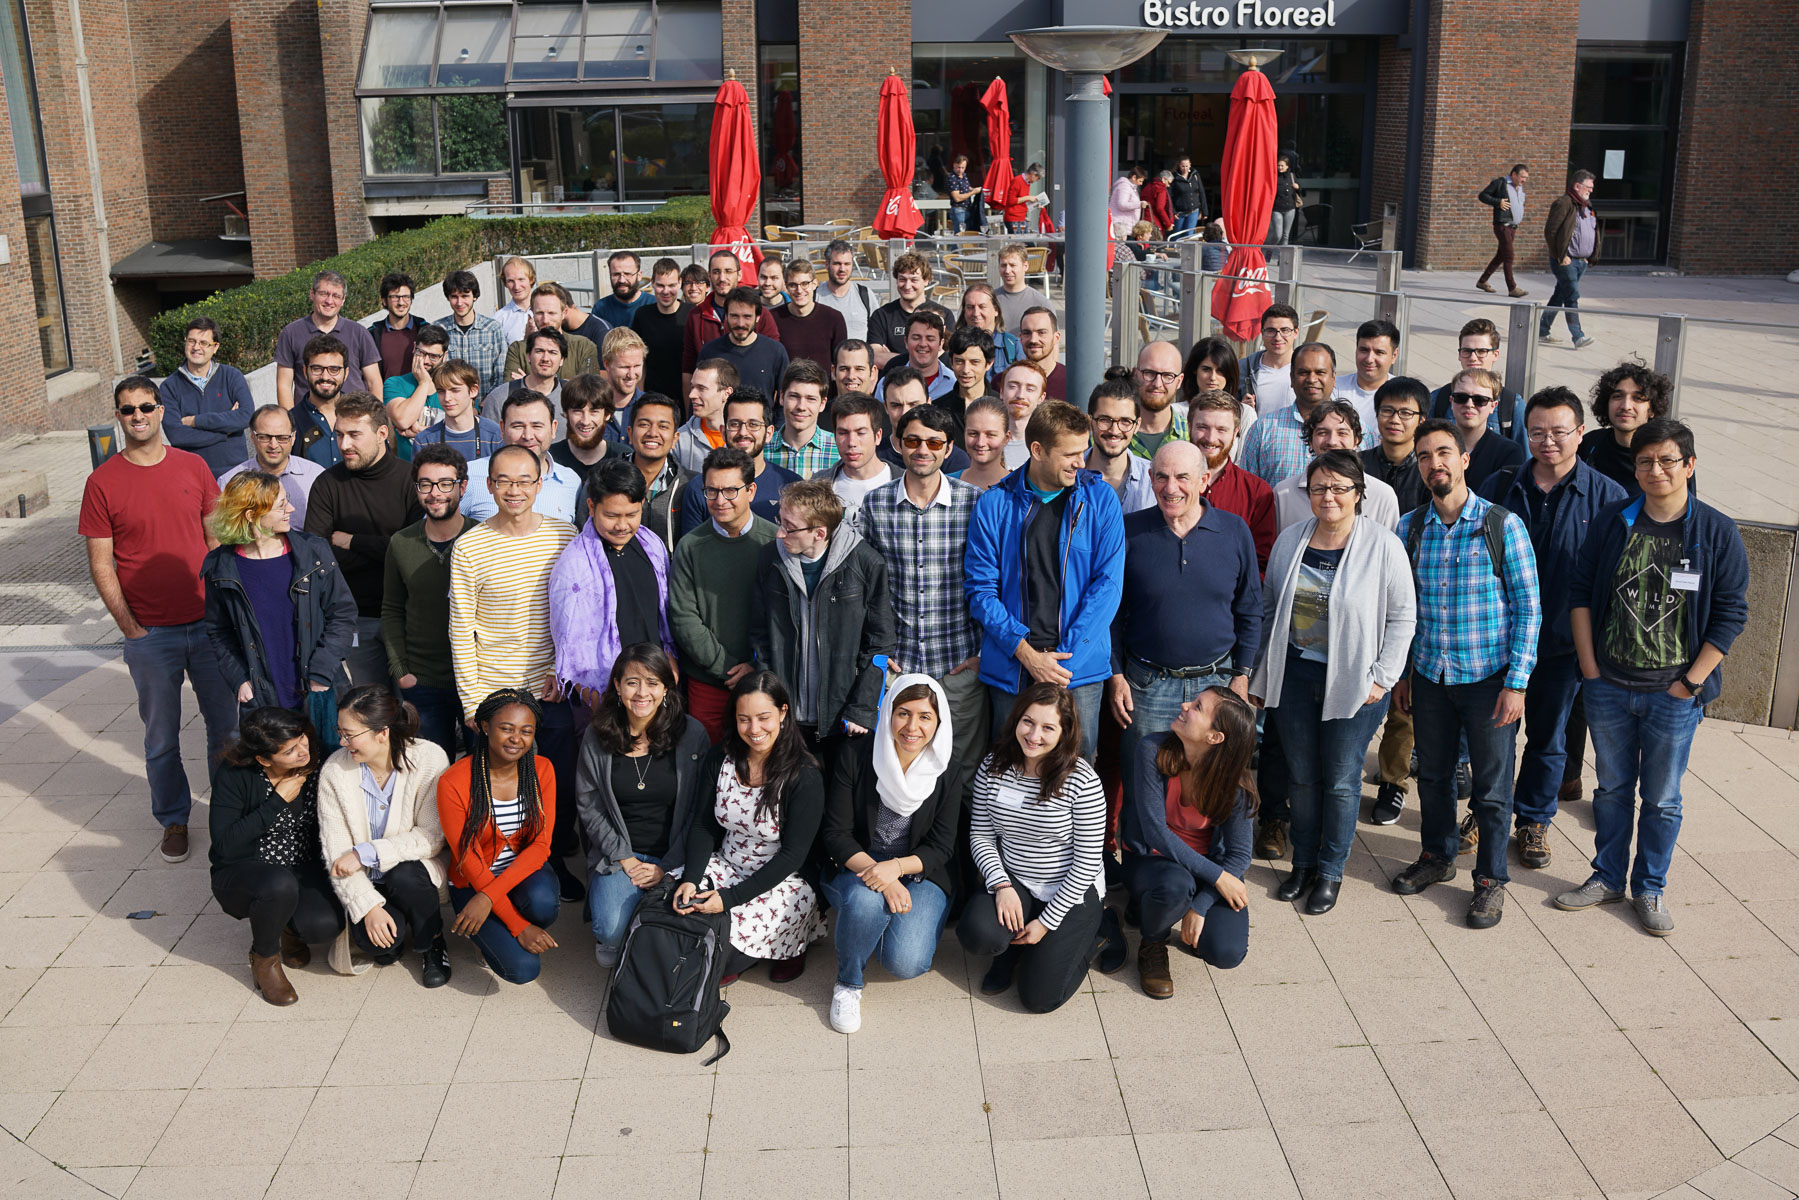
\includegraphics[height=6.5cm]{images/summer_school1}
}
\only<2>{
Munos et al., "Safe and efficient off-policy reinforcement learning", NIPS 2016 \cite{munos2016safe}
\vfill
\centering
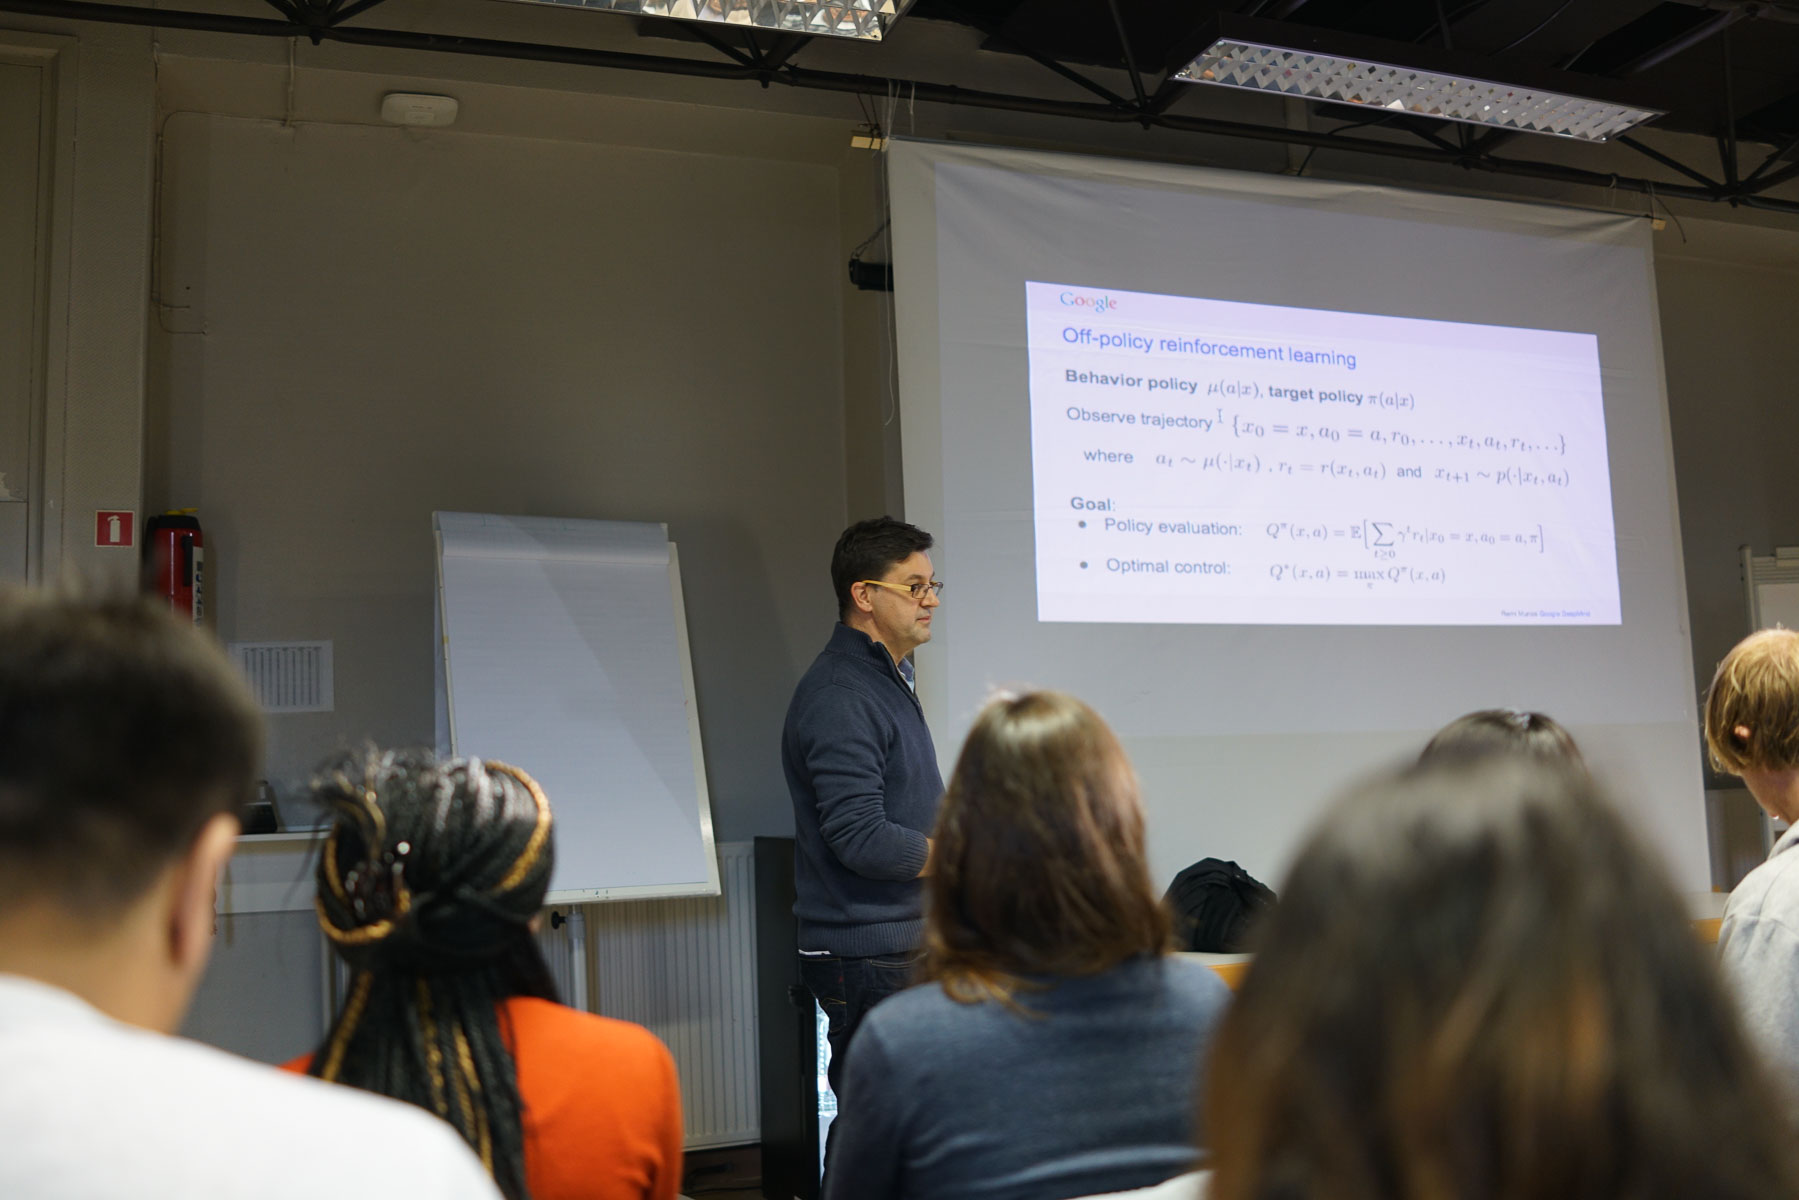
\includegraphics[height=6cm]{images/summer_school2}
}
\end{frame}

\begin{frame}
\frametitle{Syllabus}
\tableofcontents
\end{frame}

%%%%%%%%%%%%%%%%%%%%%%%%%
\section{Introduction}
%\frame{\tableofcontents[currentsection]}

\begin{frame}
\only<1>{
\frametitle{Reinforcement Learning}
\centering
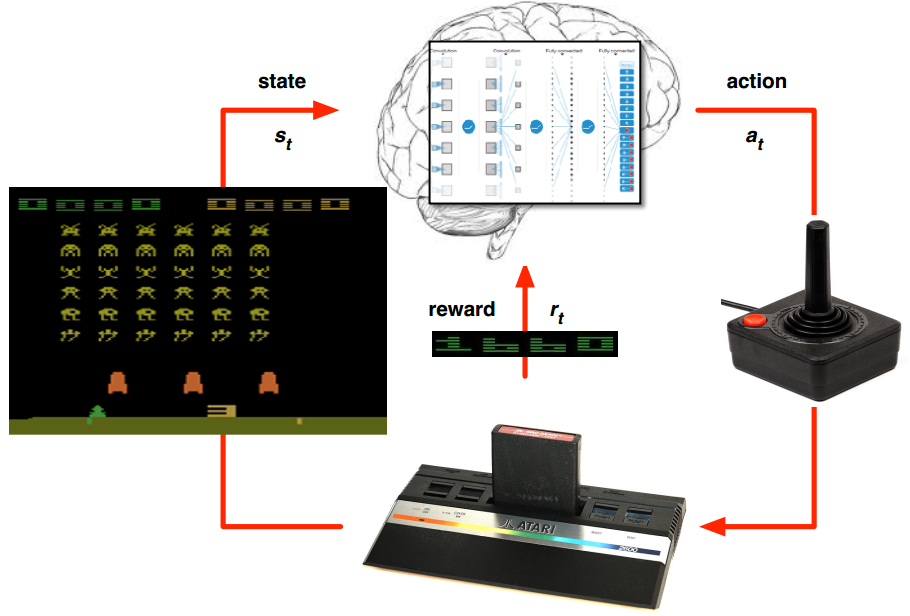
\includegraphics[height=6cm]{images/rl}
}
\only<2->{
\begin{minipage}{0.6\textwidth}
\centering
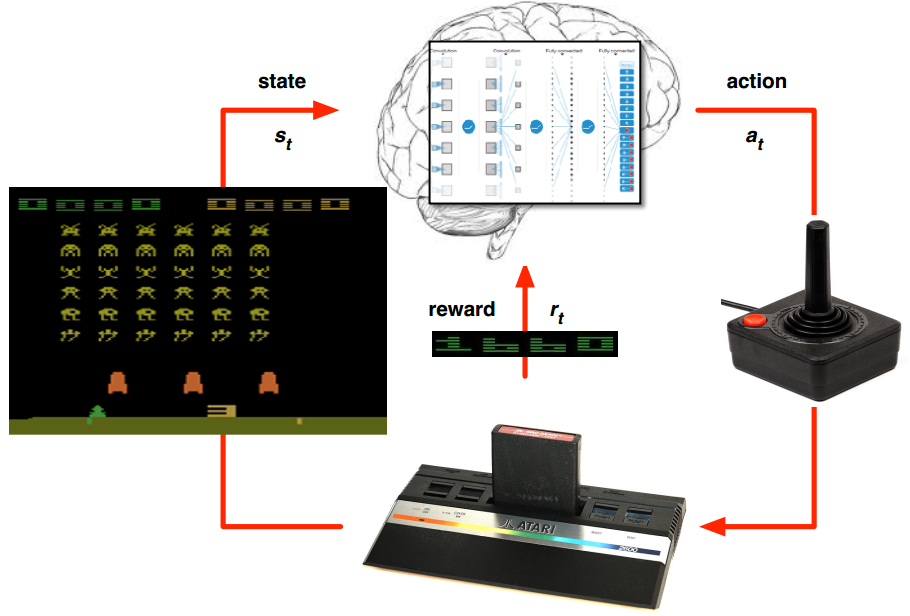
\includegraphics[height=4cm]{images/rl}
\end{minipage}%
\begin{minipage}{0.4\textwidth}
The Task
\[
	\langle\mathcal{S},\mathcal{A},\mathcal{P},\mathcal{R},\gamma,\rho\rangle
\]
\only<2>{
\begin{itemize}
\item $\mathcal{S}$: state space
\item $\mathcal{A}$: action space
\item $\mathcal{P}$: transition probabilities
\item $\mathcal{R}$: reward function
\item $\gamma$: discount factor
\item $\rho$: initial state distribution
\end{itemize}
}
\only<3->{
The agent's policy
\[
	\pi: \mathcal{S}\mapsto\Delta(\mathcal{A})
\]
}
\only<4->{
The goal
\[
	\max \sum_{t\geq 0}\gamma^t r_t
\]
}
\end{minipage}
}
\end{frame}

\begin{frame}
\frametitle{Prediction and Control}
\begin{itemize}
\item<1-> \textbf{Prediction}: measure the performance of a given policy $\pi$

\item<2> \textbf{Control}: find the optimal policy $\pi^*$
\end{itemize}
\end{frame}

\begin{frame}
\frametitle{Temporal Credit Assignment}
The effects of a choice may not be immediate 

\only<2>{$\implies$ delayed reward}
\vfill
\centering
\centerline{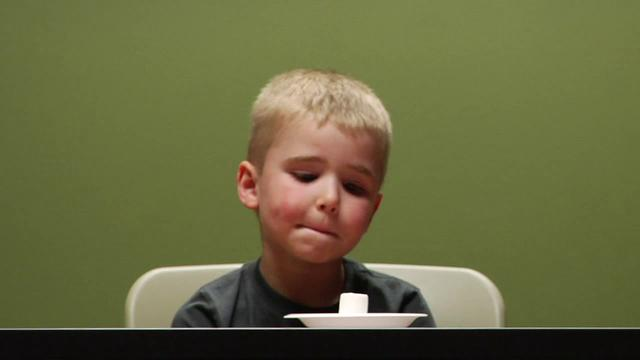
\includegraphics[height=5cm]{images/marshmallow}}
\end{frame}

\begin{frame}
\frametitle{Off-Policy Credit Assignment}
\begin{itemize}
\item<1-2> \textbf{Temporal Credit Assignment}: determine which actions, among a sequence of actions, are responsible for certain rewards
\item<2> \textbf{Off-Policy Learning}: evaluate/improve policy $\pi$ while following policy $\mu$
\item<3-> \textbf{Off-Policy Credit Assignment}: how can I give credit to choices that are not actually made?
\end{itemize}
\end{frame}
% % % % % % % % % % % % % % % % % % % % % % %

% % % % % % % % % % % % % % % % % % % % % % %
\section{Temporal Difference Learning}
\frame{\tableofcontents[currentsection]}
\begin{frame}
\frametitle{Value Function}
Bellman expectation equation:
\[
	Q^\pi(s,a) = R(s,a) + \gamma\expect{
	\shortstack{$s'\sim\mathcal{P}$\\$a'\sim\pi$}}{Q^\pi(s',a')}
\]
\pause
Bellman expectation \textbf{operator}:
\[
	\mathcal{T^{\pi}}Q = 
	R(s,a) + \gamma\expect{
		\shortstack{$s'\sim\mathcal{P}$\\$a'\sim\pi$}}{Q(s',a')}
\]
\begin{itemize}
\item<3-> $Q^{\pi}$ is the unique fixed point of $\mathcal{T^{\pi}}$
\item<4-> Contraction property: $\norm[\infty]{\mathcal{T}^{\pi}Q-Q^{\pi}} \leq \gamma\norm[\infty]{Q-Q^{\pi}}$
\end{itemize}
\end{frame}

\begin{frame}
\frametitle{Optimal Value Function}
Bellman optimality equation:
\[
	Q^*(s,a) = R(s,a) + \gamma\expect{
	s'\sim\mathcal{P}}{
	\max_{a'\in \mathcal{A}}{Q^*(s',a')}}
\]
Bellman optimality \textbf{operator}:
\[
	\mathcal{T}^*Q = 
	R(s,a) + \gamma\expect{
		s'\sim\mathcal{P}}{
	\max_{a'\in \mathcal{A}}{Q^*(s',a')}}
\]
\begin{itemize}
\item $Q^*$ is the unique fixed point of $\mathcal{T^*}$
\item Contraction property: $\norm[\infty]{\mathcal{T}^*Q-Q^*} \leq \gamma\norm[\infty]{Q-Q^*}$
\end{itemize}
\end{frame}

\hold\hold\hold
\begin{frame}
\frametitle{Prediction and Control}
\begin{itemize}
\item \textbf{Prediction}: given policy $\pi$, compute $Q^{\pi}$

\item \textbf{Control}: find $\pi^*$ such that $Q^{\pi^*}$ = $Q^*$
\end{itemize}
\end{frame}
\jump\jump

\begin{frame}
\begin{itemize}
\item<1-> Optimal \textbf{deterministic} policy:
\[
	\pi^*(s) =
	\pi_{\text{greedy($Q^*$)}}(s) \doteq \arg\max_{a'\in\mathcal{A}}Q^*(s,a') 
\]
\item<2->Maximization as a special case of expectation:
\[
	\max_{a' \in \mathcal{A}}Q
	\only<2>{^*}
	(s,a') = \expect{a'\sim
	\only<2>{\pi^*}
	\only<3>{\pi_{\text{greedy($Q$)}}}
	}{Q
	\only<2>{^*}
	(s,a')}
\]
\end{itemize}
\end{frame}

\begin{frame}
\frametitle{Temporal Difference Learning}
\begin{itemize}
\item<1-> Idea: repeatedly apply $\mathcal{T}$ to Q
\item<2-> Approximation: update Q towards a target
\only<2>{
\[
	Q(s_t,a_t) \gets Q(s_t,a_t) + \alpha\underbrace{\left[\textcolor{blue}{G_t} - Q(s_t,a_t)\right]}_{\text{TD error } \delta_t} 
\]
}
\only<3->{
\[
	\Delta Q(s_t,a_t) = \alpha\underbrace{\left[\textcolor{blue}{G_t} - Q(s_t,a_t)\right]}_{\text{TD error } \delta_t}
\]
}
\item<4> Prediction: fixed $\pi$, keep updating Q
\item<5-> Control: alternate value updates and policy updates
\[
	\pi_{k+1} = \only<6>{\textcolor{red}{(1-\epsilon)}}\pi_{\text{greedy($Q_{k}$)}} \only<6>{+\textcolor{red}{\epsilon}\pi_{\text{any}}}
\]
\only<6>{
\textbf{Increasingly greedy policy}: $\epsilon \rightarrow 0$ as $t \rightarrow \infty$
}
\end{itemize}
\end{frame}

\begin{frame}
\frametitle{Expected Sarsa}
\begin{itemize}
\item<1-> \textbf{Forward view}: look one step forward to compute the target
\[
	\Delta Q(s_t,a_t) = \alpha\left[\textcolor{blue}{r_{t+1} + \gamma\expect{a\sim\pi}{Q(s_{t+1},a)}} - Q(s_t,a_t)\right]
\]
\item<2-> \textbf{Backward view}: wait one step to update $Q(s_t,a_t)$
\begin{align*}
	\Delta Q(s_{t-1},a_{t-1}) = \alpha\left[
	\textcolor{blue}{r_t + \gamma\expect{a\sim\pi}{Q(s_t,a)}} - Q(s_{t-1},a_{t-1})\right] 
\end{align*}
\end{itemize}
\only<3>{
Convergence in tabular case \cite{van2009theoretical}
}
\end{frame}

\begin{frame}
\frametitle{Why "Expected" Sarsa?}
\begin{itemize}
\item Short answer: useful later
\item Longer answer: less variance than traditional Sarsa
\item Complete answer: Van Seijen et al. \cite{van2009theoretical}
\end{itemize}
\end{frame}

\begin{frame}
\frametitle{Temporal Credit Assignment}
How to give credit (assign value) to $(s_t,a_t)$?

\begin{itemize}
\item<1->
\textbf{Problem}: the choice of $a_t$ in $s_t$ could be rewarded at time $t+n$
\item<2->\textbf{Solution}: look at future reward!
\end{itemize}
\end{frame}

\begin{frame}
\frametitle{n-step Expected Sarsa}
Look far (n steps) in the future:
\begin{align*}
	G_t^{(n)} &\doteq r_{t+1} + \gamma r_{t+2} + \dots + \gamma^{n-1}r_{t+n}
		+ \gamma^n\expect{a\sim\pi}{Q(s_{t+n},a)} \\
		& = \textcolor{blue}{
		\only<1,4>{
		\sum_{k=1}^{n}\gamma^{k-1}r_{t+k} + \gamma^n\expect{a\sim\pi}{Q(s_{t+n},a)}
		}\only<2>{
		r_{t+1}+\gamma\expect{a\sim\pi}{Q(s_{t+n},a)}
		}\only<3>{
		\sum_{k=1}^{T-t}\gamma^{k-1}r_{t+k} + \gamma^n\expect{a\sim\pi}{Q(s_{t+n},a)}}
		}
\end{align*}
\begin{itemize}
\item<2,4> \textcolor{blue}{$G_t^{(1)}$} is a TD target: high bias, low variance
\item<3-> \textcolor{blue}{$G_t^{(T-t)}$} is a Monte Carlo target: no bias, high variance
\end{itemize}
\only<4>{
\vfill
\textbf{How can we use all future returns
\begin{itemize}
\item without storing all history
\item without delaying updates
\end{itemize}}
}
\end{frame}

%%%%%%%%%%%%%%%%%%%%%%%%%


%%%%%%%%%%%%%%%%%%%%%%%%%
\section{Eligibility Traces}

\frame{\tableofcontents[currentsection]}

\begin{frame}
\frametitle{Forward View}
Average \textbf{all} n-step targets:
\only<1,5>{
\[
	G_t^{\lambda} \doteq (1-\lambda)\sum_{n=1}^{\infty}\lambda^{n-1} G_t^{(n)}
\]
}
\only<2>{
\[
	G_t^{\lambda} = 
	(1-\lambda)
	\sum_{n=1}^{T-t-1}
	\lambda^{n-1} G_t^{(n)} + \lambda^{T-t-1}G_t^{(T-t)}
\]
}
\only<3>{
\[
	G_t^{\lambda} = 
	\textcolor{lightgray}{(1-0)
	0^0}G_t^{(1)} + 
	\textcolor{lightgray}{(1-0)\sum_{n=2}^{T-t-1}
	0^{n-1} G_t^{(n)} + 0^{T-t-1}G_t^{(T-t)}}
\]
}
\only<4>{
\[
	G_t^{\lambda} = 
	\textcolor{lightgray}{(1-1)
	\sum_{n=1}^{T-t-1}
	1^{n-1} G_t^{(n)} + 
	1^{T-t-1}}G_t^{(T-t)}
\]
}
\begin{itemize}
\item<3,5> $\lambda=0$ gives $G_t^{(1)}$, the TD target
\item<4,5> $\lambda=1$ gives $G_t^{(T-t)}$, the Monte Carlo target
\end{itemize}
\only<5>{\vfill Another way of interpolating between TD and MC}
\end{frame}

\begin{frame}
\frametitle{Backward View}
\begin{itemize}
\item Propagate TD error to past states
\item Fading memory
\end{itemize}

\vfill
\centering
\bigskip\bigskip
\centerline{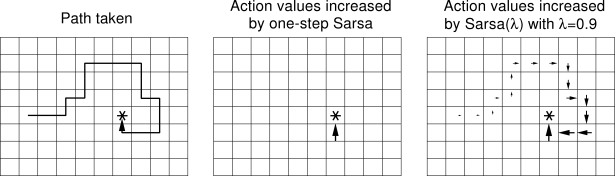
\includegraphics[height=3cm]{images/lambda}}

\end{frame}
\begin{frame}
\frametitle{Eligibility Traces}
\begin{itemize}
\item Assign a "trace" to each state-action pair
\item Set the trace to one when visited
\item All traces fade with time
\item TD update proportional to trace

\vfill
\centering
\bigskip\bigskip
\centerline{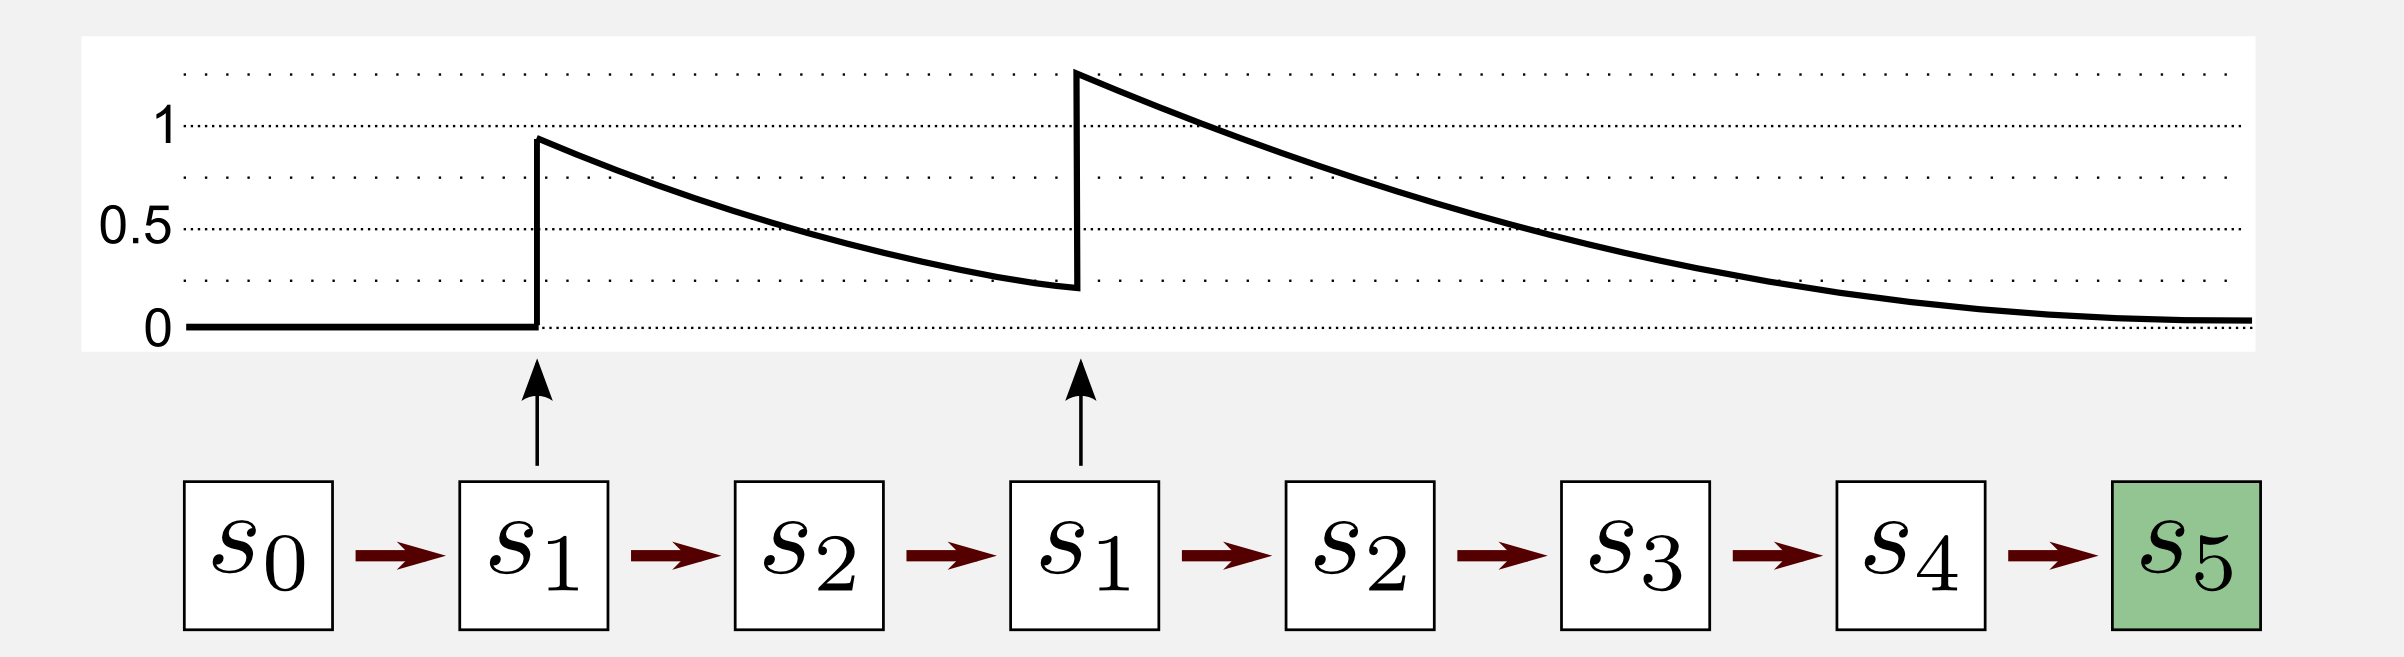
\includegraphics[height=3cm]{images/trace}}
\end{itemize}
\end{frame}

\begin{frame}
\frametitle{Accumulating Traces}
Initialization:
\[
	e(s,a) \gets 0 \text{ for all} s,a
\]
Update \textbf{all states} at each step $t$:
\begin{align*}
&
e(s,a) \gets 
\textcolor{red}{\mathbbm{1}\{s=s_t,a=a_t\}}+ 
\gamma\lambda e(s,a)
& \Delta Q(s,a) = \alpha e(s,a)(G_t^{(1)} - Q(s,a))
\end{align*}
\end{frame}

\begin{frame}
\frametitle{Back to the forward view}
Accumulating traces
\begin{align*}
	\Delta & Q(s_t,a_t) = \\ 
	&\alpha_k
	\sum_{h\geq t}\left[
	(G_h^{(1)} - Q(s_h,a_h))
	\textcolor{blue}{
	\sum_{j=t}^n(\gamma\lambda)^{h-j}
	\mathbbm{1}\left\{s_j,a_j = s_t,a_t\right\}}
	\right]
\end{align*}
\end{frame}

%%%%%%%%%%%%%%%%%%%%%%%%%

%%%%%%%%%%%%%%%%%%%%%%%%%
\section{Off-policy Credit Assignment}
\frame{\tableofcontents[currentsection]}

\begin{frame}
\frametitle{Off-Policy Learning}
Two policies:
\begin{itemize}
\item \textbf{Target} policy $\pi$: the one that is evaluated/improved
\item \textbf{Behavioral} policy $\mu$: the one that is 
used to interact with the environment
\end{itemize}
Potentially, both can change!
\vfill
Advantages: 
\begin{itemize}
\item Safe
\item Separate exploration from evaluation
\item Reuse past experience
\end{itemize}
\end{frame}

\begin{frame}
\frametitle{Importance Sampling}
Correct the update with likelihood ratios
\[
	\Delta Q(s_t,a_t) = \alpha
	\textcolor{blue}{\prod_{h\geq t}\frac{\pi(a_h\mid s_h)}{\mu(a_h\mid s_h)}}
	\left[G_t^{(n)} - Q(s_t,a_t)\right]
\]
\vfill
\only<2>{
\textcolor{red}{Issue}: high variance!
}
\end{frame}

\begin{frame}
\frametitle{Q-learning}
Approximate $\mathcal{T}^*$ directly
\[
	\Delta Q(s_t,a_t) = \alpha
	\left[ 
	\only<-2>{
	r_{t+1} +\gamma\textcolor{blue}{\max_{a\in\mathcal{A}}Q(s_{t+1},a)}
	}\only<3>{\textcolor{blue}{G_t^*}}
	 - Q(s_t,a_t)\right]
\]
\only<2->{
Implicit target policy: $\pi_{\text{greedy($Q$)}}$
}
\only<3->{
\vfill
Maximization as a special case of expectation

$\implies$ $G_t^* = G_t^{(1)}$ when $\pi$ is a greedy policy
}
\end{frame}

\begin{frame}
\frametitle{Credit Assignment}
\centering
\centerline{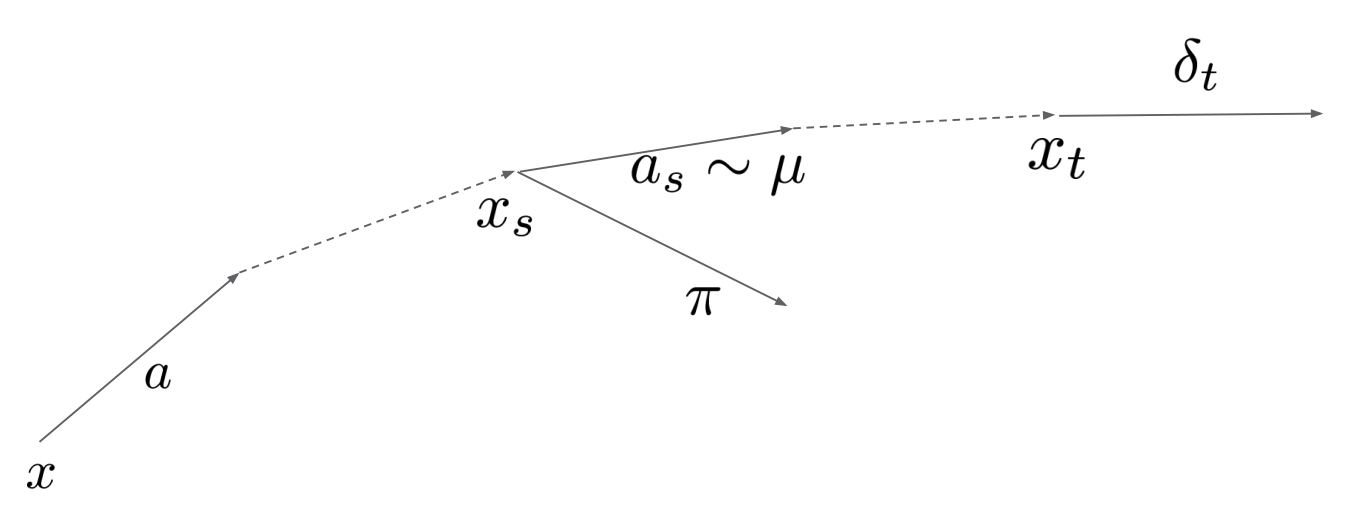
\includegraphics[height=4.5cm]{images/off_credit}}
\end{frame}

\begin{frame}
\frametitle{Watkins' Q($\lambda$)}
\textbf{Cut} the eligibility trace each time $\mu$ performs a non-greedy action

\begin{align*}
	&\text{For all $s,a$}\\
	&\qquad e \gets \gamma\lambda e + \mathbbm{1}_t \\
	&\qquad \Delta Q(s,a) = \alpha e(s,a)
	\left[G_t^* - Q(s,a)\right]\\
	&\qquad\textcolor{blue}{\text{If } a_t \neq 	\arg\max_{a'\in\mathcal{A}}Q(s_t,a')} \\
	&\qquad\qquad \textcolor{blue}{e(s,a) \gets 0} 
\end{align*}
\vfill
Credit is assigned \textbf{up to the last greedy action}

\textcolor{red}{Issues}: 
\begin{itemize}
\item Traces are cut too often
\item Convergence was an open problem since 1989!
\end{itemize}
\end{frame}

\begin{frame}
\frametitle{General Off-policy Value Update}
Back to the forward view
\only<1>{
\begin{align*}
	\Delta & Q(s_t,a_t) = \\ 
	&\alpha_k
	\sum_{k\geq t}\left[
	(G_k^{(1)} - Q(s_k,a_k))
	\textcolor{blue}{
	\sum_{j=t}^k(\gamma\lambda)^{k-j}
	\mathbbm{1}\left\{s_j,a_j = s_t,a_t\right\}}
	\right]
\end{align*}
}\only<2>{
\begin{align*}
	\Delta & Q(s_t,a_t) = \\ 
	&\alpha_k
	\sum_{k\geq t}\left[
	(G_k^{(1)} - Q(s_k,a_k))
	\textcolor{blue}{
	\sum_{j=t}^k\gamma^{k-j}
	\textcolor{red}{\lambda^{k-j}}
	\mathbbm{1}\left\{s_j,a_j = s_t,a_t\right\}}
	\right]
\end{align*}
}\only<3>{
\begin{align*}
	\Delta & Q(s_t,a_t) = \\ 
	&\alpha_k
	\sum_{k\geq t}\left[
	(G_k^{(1)} - Q(s_k,a_k))
	\textcolor{blue}{
	\sum_{j=t}^k\gamma^{k-j}
	\textcolor{red}{\left(\prod_{i=j+1}^k c_i\right)}
	\mathbbm{1}\left\{s_j,a_j = s_t,a_t\right\}}
	\right]
\end{align*}
}\only<4>{
\begin{align*}
	\Delta & Q(s_t,a_t) = \\
	&\alpha_k
	\sum_{k\geq t}\left[
	(G_k^{(1)} - Q(s_k,a_k))
	\sum_{j=t}^k\gamma^{k-j}
	\left(\prod_{i=j+1}^k \textcolor{red}{\bf{c_i}}\right)
	\mathbbm{1}_{jt}
	\right]
\end{align*}
In this formulation we call the $\textcolor{red}{\bf{c_i}}$ "traces"
}
\end{frame}

\begin{frame}
\frametitle{General Off-policy Prediction}
\begin{align*}
	\Delta Q(s_t,a_t) =
	\alpha_k
	\sum_{k\geq t}\left[
	(G_k^{(1)} - Q(s_k,a_k))
	\sum_{j=t}^k\gamma^{k-j}
	\left(\prod_{i=j+1}^k \textcolor{red}{\bf{c_i}}\right)
	\mathbbm{1}_{jt}
	\right]
\end{align*}
\begin{itemize}
\item $c_i = \frac{\pi(a_i\mid s_i)}{\mu(a_i\mid s_i)}$ 
\only<2->{$\implies$Importance Sampling!}
\item $c_i = \lambda$  
\only<3->{$\implies Q^{\pi}(\lambda)$ \cite{harutyunyan2016q}} 
\item $c_i = \lambda\pi(a_i\mid s_i)$
 \only<4->{$\implies TB(\lambda)$ \cite{precup2000eligibility}}
\end{itemize}
\end{frame}

\begin{frame}
\frametitle{$Q^{\pi}(\lambda)$}
\begin{itemize}
\item Traces: $c_i = \lambda$
\item Idea: Do not cut traces
\item Low variance
\item \textcolor{red}{Issue:} not safe

Convergence only if $\pi\simeq\mu$:
\[
	\norm[1]{\pi-\mu} \leq \frac{1-\gamma}{\lambda\gamma}
\]
\end{itemize}
\end{frame}

\begin{frame}
\frametitle{Tree-Backup $TB(\lambda)$}
\begin{itemize}
\item Traces: $c_i = \lambda\pi(a_i\mid s_i)$
\item Idea: soft cut
\item Convergence for any $\pi,\mu$
\item \textcolor{red}{Issue:} not efficient

Traces are cut unnecessarily when almost on-policy
\end{itemize}
\end{frame}

\begin{frame}
\frametitle{General Off-policy Prediction}
\begin{align*}
	\Delta Q(s_t,a_t) =
	\alpha_k
	\sum_{k\geq t}\left[
	(G_k^{(1)} - Q(s_k,a_k))
	\sum_{j=t}^k\gamma^{k-j}
	\left(\prod_{i=j+1}^k \textcolor{red}{\bf{c_i}}\right)
	\mathbbm{1}_{jt}
	\right]
\end{align*}

\begin{table}
\begin{tabular}{cll}
\toprule
Algorithm & Trace $c_i$ & Issue \\
\midrule
IS 					& $\frac{\pi(a_i\mid s_i)}{\mu(a_i\mid s_i)}$ 	& High variance\\
$Q^{\pi}(\lambda)$	& $\lambda$										& Not safe off-policy\\
$TB(\lambda)$		& $\lambda\pi(a_i\mid s_i)$						& Not efficient on-policy\\
\bottomrule
\end{tabular}
\end{table}
We want an algorithm that has \textbf{low variance}, is \textbf{safe} and \textbf{efficient}
\end{frame}

\begin{frame}
\frametitle{Safety}
\begin{theorem}[Off-policy prediction]
\label{thlabel} For any $\pi$ and $\mu$, assuming the state space is finite and all states are visited infinitely often:
\[
\text{If } \quad 0\leq c_i\leq\frac{\pi(a_i\mid s_i)}{\mu(a_i\mid s_i)} \quad \text{ then }\quad Q\rightarrow Q^{\pi}
\]
\end{theorem}
\only<2-5>{
\pause
\textit{Proof sketch: }
\pause
Define the off-policy operator $\mathcal{R}$:
\[
	\mathcal{R}Q(s,a) \doteq Q(s,a) + 
	\expect{a_t\sim\mu}{\sum_{t\geq 0}\gamma^t\left(\prod_{i=1}^{t}c_i\right)(G_t^{(1)}-Q(s_t,a_t))} 
\]
\pause

Show that $Q^{\pi}$ is the unique fixed point of $\mathcal{R}$
\pause

Show that $\norm[\infty]{\mathcal{R}Q-Q^{\pi}}\leq\gamma\norm[\infty]{Q-Q^{\pi}}$
}
\only<6>{
\vfill
\begin{itemize}
\item \textbf{Safety}: ensured
\item\textbf{Variance}: maximal when $c_i=\frac{\pi(a_i\mid s_i)}{\mu(a_i\mid s_i)}$
\item\textbf{Efficiency}: minimal when $c_i=0$ 
\end{itemize}
}
\end{frame}

%%%%%%%%%%%%%%%%%%%%%%%%%

%%%%%%%%%%%%%%%%%%%%%%%%%
\section{Retrace($\lambda$)}
\frame{\tableofcontents[currentsection]}
%%%%%%%%%%%%%%%%%%%%%%%%%
\begin{frame}
\frametitle{Retrace($\lambda$) for prediction}
\only<1>{
\begin{align*}
	& a_t \sim \mu(\cdot\mid s_t) \\
	&\Delta Q(s_t,a_t) =
	\alpha_k
	\sum_{k\geq t}\left[
	(G_k^{(1)} - Q(s_k,a_k))
	\sum_{j=t}^k\gamma^{k-j}
	\left(\prod_{i=j+1}^k \textcolor{blue}{\bf{c_i}}\right)
	\mathbbm{1}_{jt}
	\right] \\
\end{align*}
\huge{
\[
	\textcolor{blue}{c_i = \lambda\min\left\{1,\frac{\pi(a_i\mid s_i)}{\mu(a_i\mid s_i)}\right\}}
\]
}}
\only<2->{
\begin{align*}
	& a_t \sim \mu(\cdot\mid s_t) \\
	&\Delta Q(s_t,a_t) =
	\alpha_k
	\sum_{k\geq t}\left[
	(G_k^{(1)} - Q(s_k,a_k))
	\sum_{j=t}^k\gamma^{k-j}
	\left(\prod_{i=j+1}^k c_i\right)
	\mathbbm{1}_{jt}
	\right] \\
	&c_i = \lambda\min\left\{1,\frac{\pi(a_i\mid s_i)}{\mu(a_i\mid s_i)}\right\}
\end{align*}
\begin{itemize}
\item<2->\textbf{Safe} since $0\leq c_i\leq\frac{\pi(a_i\mid s_i)}{\mu(a_i\mid s_i)}$
\item<3-> \textbf{Low variance} since $c_i\leq 1$
\item<4-> \textbf{Efficient on-policy} since $c_i\rightarrow \lambda$ as $\mu\rightarrow\pi$
\end{itemize}
}
\end{frame}

\begin{frame}
\frametitle{Retrace($\lambda$) for control}
\begin{theorem}[Off-policy control]
\label{thlabel} For any $\mu_k$, if $\pi_k$ is \textbf{increasingly greedy} w.r.t to $Q_k$:
\[
\text{If } \quad 0\leq c_i\leq\frac{\pi_k(a_i\mid s_i)}{\mu_k(a_i\mid s_i)} \quad \text{ then }\quad Q_k\rightarrow Q^*
\]
\end{theorem}
\only<2-5>{
\pause
\textit{Proof sketch: }
\pause
Show that
\[
	 \norm[\infty]{\mathcal{R}Q_k - Q^*}\leq\gamma\norm[\infty]{Q_k-Q^*} + \epsilon_k\norm[\infty]{Q_k}
\]
\pause
Then $Q_k\rightarrow Q^*$ as $\epsilon_k \rightarrow 0$ 
}
\only<6>{
\vfill
Remarks
\begin{itemize}
\item No GLIE assumption on $\mu$
\item Extends to continuous action spaces
\item $c_i$ must be Markovian
\end{itemize}
}
\end{frame}


\begin{frame}
\frametitle{Solving open problems as a corollary}
\begin{align*}
	&\alpha_k
	\sum_{k\geq t}\left[
	\textcolor{blue}{(G_k^{(1)} - Q(s_k,a_k))}
	\sum_{j=t}^k\gamma^{k-j}
	\left(\prod_{i=j+1}^k 
	\textcolor{blue}{\lambda\min\left\{1,\frac{\pi(a_i\mid s_i)}{\mu(a_i\mid s_i)}\right\}}
	\right)
	\mathbbm{1}_{jt}
	\right]
\end{align*}
\only<2->{
\begin{itemize}
\item<2-> when $\pi$ is a greedy policy, $G_t^{(1)}$ is just $G_t^*$ 
\item<3->  when $\pi$ is a greedy policy, $c_i = \lambda\mathbbm{1}\left\{\mu_k(s_i) = \pi_{\text{greedy}}(s_i)\right\}$
\end{itemize}
}
\only<4>{
\vfill
\LARGE{Watkins' $Q(\lambda)$ is a special case of Retrace($\lambda$)}
\vfill
\large{Convergence of Watkins' $Q(\lambda)$ proved after 27 years!}
}
\end{frame}

\begin{frame}
\frametitle{Retrace($\lambda$) in practice}
Retrace($\lambda$) is more general than Watkins' $Q(\lambda)$
\pause
\begin{itemize}
\item<2-> $\pi_k$ and $\mu_k$ can both be increasingly greedy policies, with $\pi_k$ converging faster than $\mu_k$ $\implies $ A3C \cite{mnih2016asynchronous}
\item<3-> $\mu$ can be a snapshot of $\pi$ $\implies$ DQN with memory replay \cite{mnih2015human}
\end{itemize}
\end{frame}
%%%%%%%%%%%%%%%%%%%%%%%%%
\section{Experiments}
\frame{\tableofcontents[currentsection]}

\begin{frame}
\frametitle{Atari Games: Retrace($\lambda$) vs DQN} 
\centering
\bigskip\bigskip
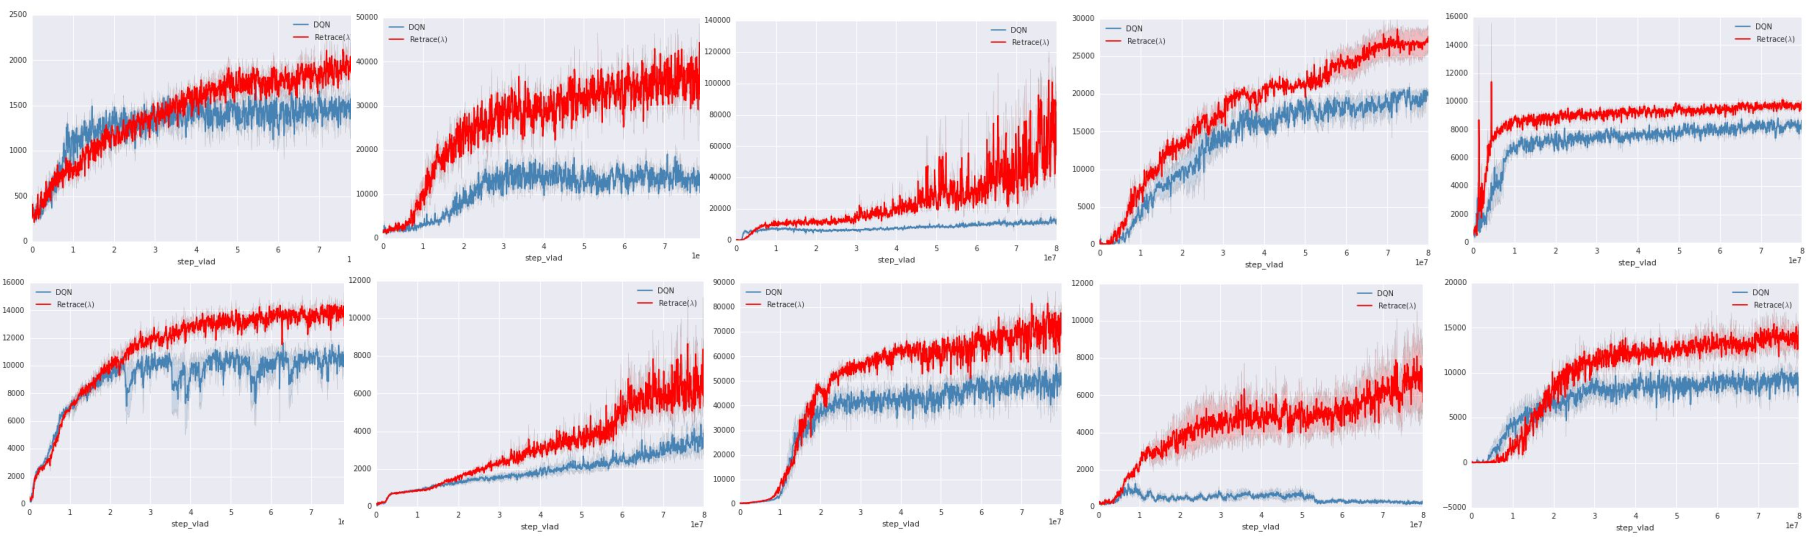
\includegraphics[height=3.4cm]{images/atari1}

Asteroids, Defender, Demon Attack, Hero, Krull,
River Raid, Space Invaders, Star Gunner, Wizard of Wor, Zaxxon
\end{frame}

\begin{frame}
\frametitle{Atari Games: Full Comparison} 
\begin{minipage}[b]{.5\textwidth}
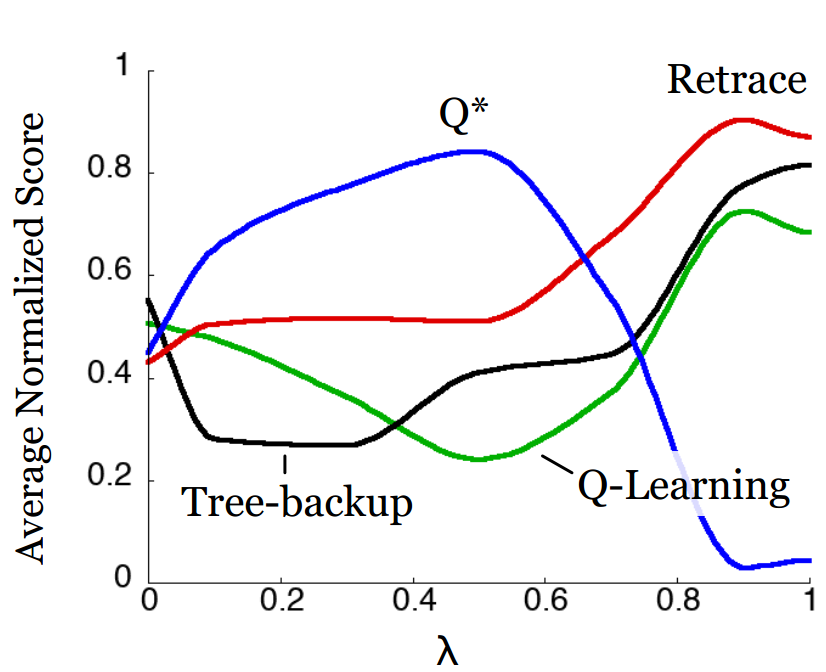
\includegraphics[height=4cm]{images/atari2}
\end{minipage}%
\begin{minipage}[b]{.5\textwidth}
\begin{tabular}{lc}
\toprule
Algorithm & Times Best \\
\midrule
DQN & 12 \\
$Q^*(\lambda)$ & 2 \\
TB($\lambda$) & 16 \\
Retrace($\lambda$) & \textbf{30} \\
\bottomrule
\end{tabular}
\end{minipage}
\end{frame}

\begin{frame}
\frametitle{Conclusion}
\begin{itemize}
\item Retrace($\lambda$) combines \textbf{off-policy} learning and \textbf{multi-step returns} in a \textbf{safe} and \textbf{efficient} way
\item In practice, it propagates sparse rewards faster than TB($\lambda$) without the convergence problems of naive Q($\lambda$)
\item With $\pi=\text{greedy(Q)}$ we have Watkin's Q-learning
\item With $\lambda=1$ we have truncated importance sampling
\item The theorems leave room for improvement
\end{itemize}
\end{frame}
%%%%%%%%%%%%%%%%%%%%%%%%%

\begin{frame}
\frametitle{Thank you!}
\centerline{\huge{Questions?}}
\centerline{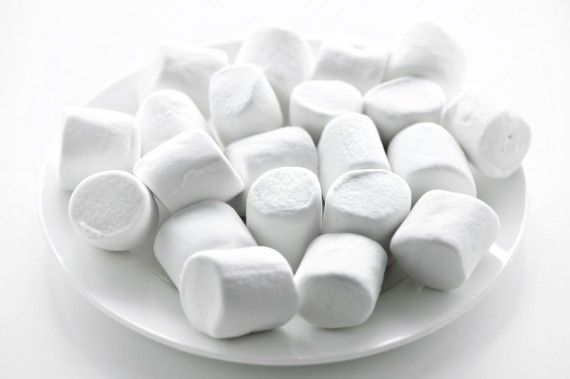
\includegraphics[4 cm]{images/marshmallow3}}
\end{frame}

\begin{frame}[allowframebreaks]
\bibliography{biblio}
\bibliographystyle{plain}
\end{frame}
% % % % % % % % % % % % % % % % % % % %

\begin{frame}
\frametitle{The Semigradient Version}
\begin{align*}
	&\boldsymbol{\theta} \gets \boldsymbol{\theta} + \alpha\delta_t \boldsymbol{e} \\
	& e \gets \nabla\hat{Q}_{\boldsymbol{\theta}}(s_t,a,_t)+\gamma\lambda \boldsymbol{e}
\end{align*}
\end{frame}

\begin{frame}
\frametitle{Accumulating Traces}
Update at step $t$:
\begin{align*}
&
\only<1>{e(s,a) \gets 
\textcolor{red}{\mathbbm{1}\{s=s_t,a=a_t\}}+ 
\gamma\lambda e(s,a)} 
\only<2>{e \gets  \textcolor{red}{\mathbbm{1}_t} + \gamma\lambda e(s,a)} 
\\
\only<1>{& \Delta Q(s,a) = \alpha e(s,a)(G_t^{(1)} - Q(s,a))}
\only<2>{& \Delta Q = \alpha e\delta_t}
\end{align*}
\end{frame}

\begin{frame}
\frametitle{Replacing Traces}
Update at step $t$:
\begin{align*}
&
e \gets \textcolor{red}{(1-\mathbbm{1}_t)}\gamma\lambda e + \mathbbm{1}_t 
\\
& \Delta Q = \alpha e\delta_t
\end{align*}
\end{frame}

\begin{frame}
\frametitle{Dutch Traces}
Update at step $t$:
\begin{align*}
& e \gets (1-\textcolor{red}{\alpha}\mathbbm{1}_t)\gamma\lambda e + \mathbbm{1}_t
\\
& \Delta Q = \alpha e\delta_t
\end{align*}
Seijen and Sutton, 2014 \cite{seijen2014true}
\end{frame}


%%%%%%%%%%%%%%%%%%%%%%%%%%%%%%%%%%%%%%%%%%%%%%%%%%%%%%%%%%%%%%%%%%%%%%%%%%%%%%%%%%%%%%%%%%%%%%%%%%%%%%%%%%%%%%%%%%

\end{document} 
